\chapter{Návrh aplikace} \label{chap:app-design}
% Jedním z cílů této části práce je obecný návrh systému pro vyhledávání osob a pracovišť dle jejich kompetencí.
V následující kapitole rozebereme zevrubně návrh systému pro vyhledávání osob a pracovišť dle kompetencí. Budeme postupovat od nejobecnějšího (cíle a požadavky) ke konkrétnímu (případy užití, volba architektury). Stále se budeme pohybovat po technologicky nezávislé rovině, tu rozebereme až v následující kapitole při popisu prototypu. Stejně tak otázky reprezentace jsou na této rovině irelevantní, přestože ty jsme již rozhodli.
% Přestože jsme v první části této práce zmínili jako vhodnou reprezentaci znalostí ontologie, v této kapitole 
% Dokonce je na místě se v této kapitole odstínit i od dříve zmíněných ontologií, jelikož architektura aplikace by na takových věcech neměla být závislá.

% [TODO: Dekompozice problému budeme na to dbát při návrhu architektury pozdějšího systému - musíme být schopni nahradit moduly --> to by se hodilo na to navázat v úvodu té sekce Architektura]

\section{Podnět vzniku aplikace} %(to by mělo být zjevné již od začátku práce!)
Idea této aplikace pro vyhledávání osob dle kompetencí vznikla na FEL ČVUT, konkrétně u pana Ing. Martina Klímy, Ph.D.\par
Pan Klíma měl představu, že by měla na webových stránkách FEL vzniknout sekce, kde by třetí strany, konkrétně průmysloví partneři, mohli vyhledávat osoby dle jejich kompetencí. Partneři by později mohli kontaktovat daného člověka případně jeho vedoucího pracovníka, pokud by měli zájem s ním více spolupracovat. Tímto způsobem by tedy fakulta nabízela pracovníky a jejich kompetence širší veřejnosti, samozřejmě s jejich souhlasem.\par
První práce, která vznikla na toto téma je bakalářská práce Romana Kuchára z roku 2016. Pan Kuchár problematiku řešil poměrně přímočaře, způsobem, který pan Klíma popsal. \cite{kuchar} Po analýze kódu lze postup shrnout do následujících kroků:
\begin{enumerate}
    \item \textbf{Uživatel} zadá klíčové slovo tzv. expertise
    \item \textbf{Systém} nalezne výskyt tohoto slova v článcích v systému V3S (v titulu, klíčových slovech či abstraktu)
    \item \textbf{Systém} na základě hodnocení nalezených publikací (tzv. rivs) ohodnotí nalezené autory, přitom vezme v úvahu i míru jejich participace
    \item \textbf{Systém} vrátí seznam nalezených autorů seřazený dle jejich vypočteného hodnocení
\end{enumerate}
Řešení pana Kuchára v kontextu naší práce spadá pod varianty bez znalostní báze a bez práce se znalostmi vůbec (což nemusí být nutně špatně). V kapitole č. \ref{future} se zmíníme o řešeních tohoto typu.\par
Cílem této práce je celou problematiku prověřit zevrubněji (jak je vidět z první části této práce). Při návrhu aplikace budeme vycházet z požadavků/cílů, které definoval v úvodu pan Klíma a z požadavků, které jsme při této práci dále identifikovali.\par
Existuje mnoho dalších možností, jak vzniklou aplikaci obohatit o další užitečné funkce. V této práci však budeme pracovat se základními požadavky, pomocí kterých budeme tvořit jádro aplikace.
\section{Vymezení této práce}
\subsection{Rozsah řešené problematiky}
Na úvod upřesníme, čím se budeme v následujících sekcích zabývat. Celou problematiku vyhledávání osob a pracovišť dle jejich kompetencí, která vyplývá z pokynů k vypracování této práce, jsme v předchozí části práce zúžili na vyhledávání osob a pracovišť dle znalostí (viz kapitola \ref{chap:data_representation}). Pro účely následujících kapitol zúžíme celý problém pouze na vyhledávání osob dle znalostí.\par
Primárním důvodem je, že z definice kompetence pracoviště (kapitola \ref{sec:terms}) vyplývá, že je složena z kompetencí osob. Vyřešíme-li tedy problém vyhledávání osob dle kompetencí, stěžejní část problému vyhledávání pracovišť dle kompetencí vyřešíme též. Se znalostmi je to v tomto kontextu stejné jako s kompetencemi.\par
% Sekundárním důvodem je rozsah této práce, který je dostačující i bez dalšího případu užití.
\subsection{Rozsah navrženého systému}
Jak jsme zmínili výše, v následující kapitole rozebereme návrh aplikace pro vyhledávání dle kompetencí. Důležité je zmínit, že navrhneme celý systém až na část, která se zabývá transformací dat. Transformací dat, kterou jsme popsali v předchozí kapitole (č. \ref{chap:data-sources-analysis}), se vzhledem k rozsahu problematiky zabývat nebudeme. Zmíníme jí však v kapitole budoucí práce (č. \ref{future}), jelikož je to problematika, která musí být před nasazením navrženého systému vyřešena - bez dat jej nelze využívat.\par
\subsection{Rozsah implementovaného prototypu}
V následující kapitole (č. \ref{chap:implementation}) se budeme zabývat prototypem, který jsme v rámci naší práce implementovali. Účelem implementační části této práce je dokázat, že řešení navržené v této kapitole je možné použít a že skutečně může po dalších rozšířeních fungovat v praxi. Nejedná se tedy o kompletní implementovaný systém. V úvodu příští kapitoly zmíníme konkrétně rozsah obou částí prototypu.

% V předchozí kapitole (\ref{chap:data-sources-analysis}) jsme rozebrali datové zdroje osob, pracovišť a znalostí dostupné na FEL ČVUT. V rámci návrhu aplikace
% V následující kapitole se budeme
% V rámci této práce na tuto část již nenavážeme řešením transformace dat do ontologií a tak dále. To je velmi komplikovaná problematika, vhodná pro další zkoumání, v rámci další práce. V této práci budeme pro další kapitoly předpokládat, že data máme připraveny ve zvolené struktuře.
% Navrhneme kompletní systém, implementujeme prototyp...
\section{Požadavky}
\subsection{Základní business požadavek}
Základní business požadavek, který naše aplikace musí splnit je: \textit{Umožnit třetím stranám fakulty (firmám, výzkumným centrům a jiným) vyhledávát pracovníky FEL ČVUT dle jejich kompetencí, s jejich svolením.}
\subsection{FURPS+ analýza} \label{furps}
\subsubsection{Funkce}
\begin{itemize}
    \item Vyhledat seznam pracovníků FEL seřazených dle jejich vypočtené síly znalosti na základě zadaného klíčového slova (libovolného nebo zvoleného z definované množiny slov)
\end{itemize}
% dobrovolné požadavky (pro lepší práci s API, další možnosti)
% - CRUD nad entitami - osoby, znalosti, pracoviště
% - pro definovaného člověka nalézt jeho znalost v definovaném odvětví
% - ...
\subsubsection{Použití}
\begin{itemize}
    \item Část aplikace, do které bude přistupovat koncový uživatel, musí být dohledatelná pomocí běžných vyhledávačů dle klíčových slov (minimálně google a bing)
    \item Část aplikace, do které bude přistupovat koncový uživatel, musí být jednoduchá k použití - očekávají se uživatelé, kteří jsou gramotní při běžné práci s počítačem (textové procesory, práce s prohlížečem a webovými formuláři)
    \item Koncový uživatel aplikace musí mít k dispozici příručku (nejlépe interaktivní formou přímo v rozhraní)
    \item Aplikace musí být dostupná bez přihlášení, login se toleruje jen pro případná speciální administrátorská práva
    \item API musí být kompletně zdokumentováno pro budoucí použití jinými programátory
\end{itemize}
\subsubsection{Spolehlivost a výkon}
Aplikace nemá žádná zvláštní omezení na spolehlivost a výkon. Předpokládá se spolehlivost na úrovni ostatních nekritických aplikací univerzity - 98\%. Aplikace nemá speciální požadavky na výkon.
\subsubsection{Údržba}
\begin{itemize}
    \item Použitá technologie musí být kompatibilní s budoucím správcem aplikace (FEL)
    \item Aplikace bude koncipována jako webová, ne nativní
\end{itemize}
\subsubsection{Bezpečnost}
Data, která budou dostupná z aplikace, mohou být pouze data veřejně dostupná.
% data o zaměstnancích, jelikož budou k dispozici bez přihlášení. V opačném případě musí aplikace umožnit sbírání souhlasů s využitím osobních údajů.
\subsubsection{Implementace}
Architektura aplikace musí být modulární. Celý problém vyhledávání osob dle kompetencí, reprezentace znalostí a vše okolo má velmi mnoho možných přístupů k řešení. Architektura aplikace musí umožňovat jednoduchou výměnu jednotlivých modulů za jiné implementace.
\subsection{Případy užití}
% Případů užití navrhované aplikace není mnoho, na druhou stranu je poměrně komplikované je realizovat. Konkrétně hlavní případ užití aplikace (UC1 - Vyhledat osoby na FEL dle kompetencí) a jeho část, kdy systém musí vyhledat znalost a osoby, je v podstatě jádrem celé této práce.\par
\subsubsection{Aktéři}
Aplikace bude ze své podstaty otevřena široké veřejnosti. Hlavním uživatelem tedy bude \textit{nepřihlášený uživatel}.
\subsubsection{UC1 - Vyhledat osoby na FEL dle kompetencí} \label{UC1}
\paragraph{Scénář:}
\begin{enumerate}
    \item \textbf{Uživatel} zadá klíčové slovo (libovolné nebo vybrané z definované množiny slov)
    \item \textbf{Systém} nalezne na základě zadaného klíčového slova kompetenci (reprezentovanou libovolným způsobem) a osoby, které se k ní vztahují. Následně \textbf{systém} vypočítá/vyhledá sílu kompetence pro každou nalezenou osobu. Nakonec tento seřazený seznam osob vrátí uživateli. Neexistuje-li žádná osoba s touto kompetencí, systém vrátí uživateli prázdný seznam. 
\end{enumerate}
Seznam vrácený uživateli může být parametrizován pomocí offset a limit. \textbf{Limit} určuje počet výsledků, který má být vrácen. \textbf{Offset} potom určuje pořadové číslo prvního řádku z výsledku, který má být uživateli vrácen.
\subsection{Wireframy}
\subsubsection{W-UC1 - Vyhledat osoby na FEL dle kompetencí}
\begin{figure}[htbp!]
	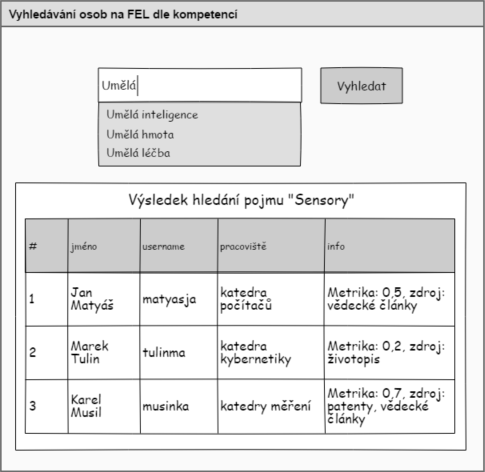
\includegraphics[width=0.9\linewidth]{img/W-UC1.png}
	\caption{Obrázek k W-UC1 (zdroj autor)}
	\label{fig:w-uc1}
\end{figure}
 \noindent \textbf{Vyhledávací pole} - zajišťuje uživatelský vstup, může být implementováno jako prosté textové pole s omezením na délku, či jako výběr s možností vyhledání\par
\paragraph{Tabulka s výsledkem obsahuje sloupce:}
\begin{itemize}
    \item Jméno - celé jméno osoby včetně titulů
    \item Username - username v rámci FEL ČVUT (slouží též jako email, po přidání domény)
    \item Pracoviště - název a kód pracoviště
    \item Info - libovolné informace, relevantní pro podložení vyhledaných informací a podobně
\end{itemize}

\section{Architektura aplikace}
Zkoumaný problém není složitý počtem funkcí, ale náročností jednotlivých celků. Tato náročnost se dosti odráží na architektuře celé aplikace. Aplikace může být integrována s různými typy úložišť a modularita musí zajistit jednoduché nahrazování jednotlivých částí (vyplývá z FURPS+ analýzy (\ref{furps})).
\subsection{Klient, Server}
Infrastruktura FEL ČVUT sestává primárně z webových aplikací. Tato platforma bude dodržena i v našem případě - viz FURPS+ (\ref{furps}).\par
Hlavní část aplikace je koncipována jako server s definovaným rozhraním, skrz které budou dostupné výše zmíněné případy užití. S rozhraním bude komunikováno pomocí HTTP protokolu. V této době jsou nejpoužívanějšími komunikačními přístupy: REST \cite{REST} a GraphQL \cite{GRAPHQL}, volba záleží na konkrétní realizaci.\par
Součástí této práce bude i klientská aplikace, na které demonstrujeme průběh komunikace se serverovou částí aplikace.
\subsection{Architektura}
Slovo architektura se v dnešní době používá v nesčetně významech. V praxi to často jde tak daleko, že již není ani zjevné, co má řečník opravdu na mysli.\par
Jak píše Martin Fowler, i když cynicky, ve své knize \textit{Patterns of Enterprise Application Architecture}, slovo architektura se používá, když lidé chtějí upozornit na něco, co je opravdu důležité. \cite{fowler-patterns}\par
Fowler poukazuje na to, že architektura je ve své podstatě rozpad systému na části a následné nastavení pravidel komunikace mezi těmito částmi. Možných architektonických vzorů je nespočet a klíčovým parametrem je nejčastěji dispozice ke změnám. Jinými slovy je klíčové, jestli se daná část aplikace bude v průběhu času měnit a jestli je tomu vybraná architektura dobře přizpůsobená. \cite{fowler-patterns}\par
V jedné aplikaci může být použito více architektonických vzorů \cite{fowler-patterns}. Dá se říct, že v tomto případě funguje přísloví \textit{účel světí prostředky}, pokud tedy daný vzor v dané situaci funguje správně, byl použit správně. Neexistuje samozřejmě jen jedno možné řešení, obzvlášť vezmeme-li v úvahu, jak rychle se technologie vyvíjí.\par
Architektura je subjektivní a je vždy závislá na systému i vývojovém týmu, který daný systém vyvíjí. \cite{fowler-patterns} Motivací, proč řešit architekturu, je nejčastěji potřeba vyhnout se pozdějším změnám, které jsou často časově náročné až likvidační.
\subsection{Výběr architektury}
Než přistoupíme k architektuře, která se nejvíce hodí pro náš systém, musíme shrnout úkoly, které aplikace bude plnit a data, která bude zpracovávat.
\paragraph{Data:}
\begin{itemize}
    \item Aplikační data - uživatelé aplikace, jejich práva, další data týkající se přídavných funkcí vyhledávače (historie hledání a podobně) 
    \item Zpracovávaná data - znalosti, osoby, pracoviště
\end{itemize}
\paragraph{Úkoly:}
\begin{itemize}
    \item Autorizace, autentizace, účty, cachování, další možnosti pro uživatele případně správce vyhledávače
    \item Poskytování všech druhů dat (CRUD operace)
    \item Uchovávání dat
    \item Zpracování znalostí, osob, pracovišť - agregace, reprezentace, operace při vyhledávání a jiné
    \item Získávání znalostí, osob, pracovišť
\end{itemize}
Ne všechny výše zmíněné úkony musí plnit první verze aplikace, dokonce nemusí existovat jen jediná aplikace, která celý problém bude řešit. Nicméně, jak jsme výše zmínili, je třeba počítat s budoucím nahrazováním jednotlivých částí a hledáním nových způsobů. Při volbě architektury tedy musíme počítat se všemi funkcemi, které nyní jsme schopni odhadnout.\par
Z FURPS+ analýzy (\ref{furps}) plynou zároveň požadavky na architekturu týkající se hlavně technologie a modularity vybraného řešení.\par
Systém není příliš složitý, co se týká počtu funkcí. Naproti tomu se však staví jeho komplexita vzhledem k integracím s jinými systémy (různé druhy databází, získávání dat z jiných API), která bude při volbě architektury klíčová. Z hlediska komplexity systému bychom tedy naší aplikaci nepovažovali za enterprise aplikaci v plném rozsahu, jak jí definuje Fowler ve své knize. Fowler píše, že enterprise aplikace obvykle zahrnují větší množství dat a paralelní přístup mnoha uživatelů  \cite{fowler-patterns}, což u naší aplikace nepředpokládáme. Naopak v ohledu integrace s jinými systémy se jedná o komplexní (enterprise) aplikaci a je třeba jí tímto způsobem navrhnout a spravovat.\par
Při tvorbě komplexnějších aplikací je jedním ze základních přístupů tzv. vrstvení (angl. layering) \cite{fowler-patterns}, rozhodli jsme se jej použít i v našem případě. Nejedná se o architektonický vzor, spíše o styl nebo přístup k tvorbě aplikací. Hlavním úkolem při tvoření vrstev je samozřejmě definice toho, za co každá vrstva zodpovídá \cite{fowler-patterns} a jak jsou nastavené závislosti mezi jednotlivými vrstvami.\par
Z počátku jsme zamýšleli použít vrstevnatou architekturi dle Browna (tabulka č. \ref{tab:brown}). 
\begin{table}[htbp!]
\begin{ctucolortab}
\begin{tabularx}{0.3\linewidth}{l}
                Prezentace \\ \hline
                Kontroler, mediator \\ \hline
                Doména \\ \hline
                Mapování \\ \hline
                Zdroj
\end{tabularx}
\end{ctucolortab}
	\caption{Tabulka vrstev architektury dle Browna (zdroj \cite{fowler-patterns}, přeložil autor)}
	\label{tab:brown}
\end{table}
Jak píše Fowler, v případě \textit{Brownovy architektury} můžeme vzít v úvahu další varianty. Můžeme vzít hlavní tři vrstvy a mezivrstvy dodávat v případě přílišné komplexity systému. \cite{fowler-patterns}\par
V takto vrstevnaté architektuře je komunikace mezi vrstvami typicky nastavena jedním směrem, tzn. že vrstvy mohou volat buď všechny vrstvy níže, nebo jen jednu o patro níž. 
% [obrázek beyond - classic layered architecture]
\par
\textit{Brownovu architekturu} můžeme klasifikovat jako klasickou vrstevnatou. Architektury tohoto typu mají jednu značnou nevýhodu, kterou je přílišné provázání celého systému (angl. coupling) s datovými zdroji. Datové zdroje (databáze, soubory, webové služby) jsou totiž typicky svázány přímo s aplikační logikou, přes definované mapování (viz předposlední vrstva v tabulce č. \ref{tab:brown}).\par
\noindent Na tento nedostatek poukázal ve své práci Jeffrey Palermo, který konkrétně zmiňuje:
\begin{quote}
    Kámen úrazu je v tomto případě fakt, že aplikace je postavená okolo dat a ostatní infrastruktury. Jelikož je aplikace takto provázána, tak pokud se změní přístup k datům, externí služba a podobně, musí se změnit i business logika aplikace. \cite{palermo}  (přeložil autor)
\end{quote}
% [TODO: obrázek od Jeffreyho]
Odstínění částí jako je databáze, které Palermo nazval infrastrukturou, je i pro nás velmi klíčové.
% Je tomu tak, protože není jasné, kolik způsobů bude třeba v budoucnu vyzkoušet, aby náš systém fungoval efektivně. V rámci této práce implementujeme jeden z možných způsobů.
\par
Palermo staví na místo toho jiný typ architektury. Architekturu, kterou nazval cibulová architektura (angl. Onion architecture). Tato architektura podle něj lépe pracuje s provázaností programu \cite{palermo} a tedy se i více hodí pro náš případ. Palermo ve své práci dodává, že se nejedná o zcela nový přístup, on je ale ten, kdo jej pojmenoval a propagoval.\par
\begin{figure}[htbp!]
	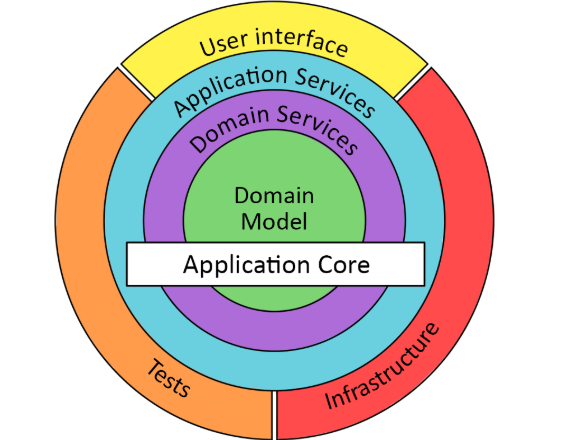
\includegraphics[width=0.7\linewidth]{img/onion.png}
	\caption{Cibulová architektura (zdroj \url{https://dzone.com/})}
% 	 articles/ onion-architecture-is-interesting
	\label{fig:onion}
\end{figure}
Cibulová architektura (obr. č. \ref{fig:onion}) se vyznačuje především tím, že infrastruktura je vždy považována za vnější vrstvu (na obrázku \textit{Tests, User interface a Infrastructure}). Ve středu je tzv. doménový model (na obrázku \textit{Domain Model}), který v podstatě reprezentuje entity reálného světa, které v systému používáme \cite{palermo} ve formě datových struktur (objektů). Doménový model je jediná část aplikace, která je závislá pouze sama na sobě. Na tuto vrstvu navazuje libovolný počet dalších vrstev. Obvykle zde bývá vrstva, která se zabývá manipulací s doménovým modelem - ukládání a získávání (na obrázku \textit{Domain Services}). Tato vrstva se zde vždy nachází ve formě rozhraní, implementace tohoto rozhraní je totiž až součást vyšší vrstvy infrastruktury. Nad těmito vrstvami se může nacházet další vrstva aplikační logiky, kde se již řeší business logika aplikace (na obrázku \textit{Application Services}). Okolo potom stojí infrastruktura (DB, soubory, webové služby), testy, uživatelské rozhraní. Závislosti mezi vrstvami jsou vždy koncipovány, tak aby jedna vrstva závisela pouze na vrstvách, které jsou v obrázku č. \ref{fig:onion} blíže ke středu. \cite{palermo}\par
Při použití této architektury bychom v našem případě mohli vyhovět požadavku na jednoduché provádění změn v infrastruktuře. To je totiž právě důvod, proč je cibulová architektura navržena tímto způsobem. Dle Palerma se totiž nejčastěji mění právě infrastruktura a tato architektura jí proto staví do vnější vrstvy, jejíž změny neovlivní doménu ani business logiku. \cite{palermo}\par
Cibulová architektura je tedy pro náš případ nejvhodnější, proto jsme se rozhodli pro jednu z variant této architektury - tzv. hexagonální architekturu.

\section{Hexagonální architektura - Porty a adaptéry}
Robert C. Martin (Uncle Bob) se ve své práci zmiňuje o několika architekturách, mezi nimi i cibulová a hexagonální, a shrnuje jejich společné znaky. Zmiňuje, že obě architektury mají stejný cíl, a to je oddělení zájmů (angl. separation of concerns), o tom se mimochodem zmiňuje i Jeffrey Palermo \cite{palermo}. Obě architektury tohoto dosahují rozdělením systému do vrstev a obě architektury oddělují business část aplikace od infrastruktury. \cite{uncle-bob} Systém, který staví na těchto principech je obvykle nezávislý na knihovnách, dobře testovatelný, architektonicky nezávislý na typu UI, typu databáze i na jiných externích systémech. \cite{uncle-bob}.\par
Hlavní myšlenku hexagonální architektury zformuloval Alistair Cockburn. Ve svém článku se odkazuje na stejné principy, které jsou zmíněny výše u Palerma. Nejvíce se opírá o myšlenku, že problematika poskytování dat a získávání dat je ve své podstatě totožná a není třeba jí řešit různými způsoby. Cockburn si všiml, že v jiných architekturách (například v Brownově zmíněné výše) je častým jevem, že při návrhu systému se s těmito dvěma problematikami zachází různým způsobem. Architektura se jinak nazývá též porty a adaptéry, protože ty se staly nástrojem, jak se vypořádat s poskytování a získáváním dat. \cite{cockburn}\par

\begin{itemize}
    \item \textbf{Porty} jsou vstupními body, které jádro aplikace poskytuje.\cite{bergen}
    \item \textbf{Adaptéry} slouží jako most mezi aplikací a službami, které jsou potřeba pro její chod. Vždy patří ke specifickému portu. \cite{bergen}
\end{itemize}
Přestože se architektura snaží řešit porty a adaptéry univerzálně, vzhledem k existenci různých aktérů v rámci systému, i porty a adaptéry se dále dělí. \cite{cockburn} \par
Aktéři jsou buď primární či sekundární. Primární aktér řídí aplikaci (typicky uživatel, ale například i test) - na obr. č. \ref{fig:hexagonal} \textit{Driver Side}. Sekundární aktér je řízen aplikací (typicky databáze, resp. databázový repositář) - na obr. č. \ref{fig:hexagonal} \textit{Driven Side}. \cite{cockburn} \cite{hexagonal-this}\par
% Porty a adaptéry se stejným způsobem dělí na primární a sekundární (na obrázku č. \ref{fig:dependency-hexagon} lze vidět, jak fungují v architektuře závislosti, které s dělením portů a adaptérů souvisí).
\begin{figure}[H]
	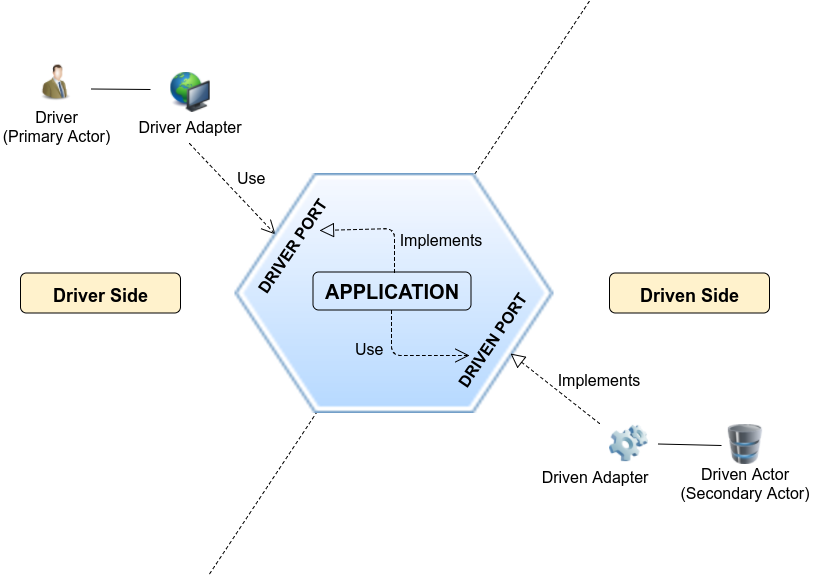
\includegraphics[width=\linewidth]{img/hexagonal-scheme.png}
	\caption{Hexagonální architektura (zdroj \cite{hexagonal-this})}
	\label{fig:hexagonal}
\end{figure}
\newpage
\begin{itemize}
    \item \textbf{Dělení portů}
        \begin{itemize}
            \item Primární - tvoří aplikační rozhraní nabízené aplikací (na obrázku č. \ref{fig:dependency-hexagon} API), jsou volány primárními adaptéry \cite{bergen} \cite{hexagonal-this}
            \item Sekundární - tvoří rozhraní vyžadované aplikací (na obrázku č. \ref{fig:dependency-hexagon} SPI), jsou volány jádrem aplikace \cite{bergen} \cite{hexagonal-this}
        \end{itemize}
    \item \textbf{Dělení adaptérů}
        \begin{itemize}
            \item Primární - volají primární porty, například testy aplikační logiky, kontroler pro komunikaci s UI (na obrázku č. \ref{fig:dependency-hexagon} Controller jako příklad) \cite{bergen}
            \item Sekundární - implementují sekundární porty, například databázové repozitáře, nebo mockovací knihovny (na obrázku č. \ref{fig:dependency-hexagon} Persistence jako příklad)\cite{bergen}
        \end{itemize}
\end{itemize}
Na obrázku č. \ref{fig:dependency-hexagon} je navíc dobře vidět, že celá aplikace je svázána doménovým modelem (na obrázku Domain Objects). \par
% Primárním adaptérům se někdy též říká řídící (angl. driver), naopak sekundárním se říká řízené (angl. driven), viz obr. č. \ref{fig:hexagonal} \cite{cockburn}.\par
\begin{figure}[H]
	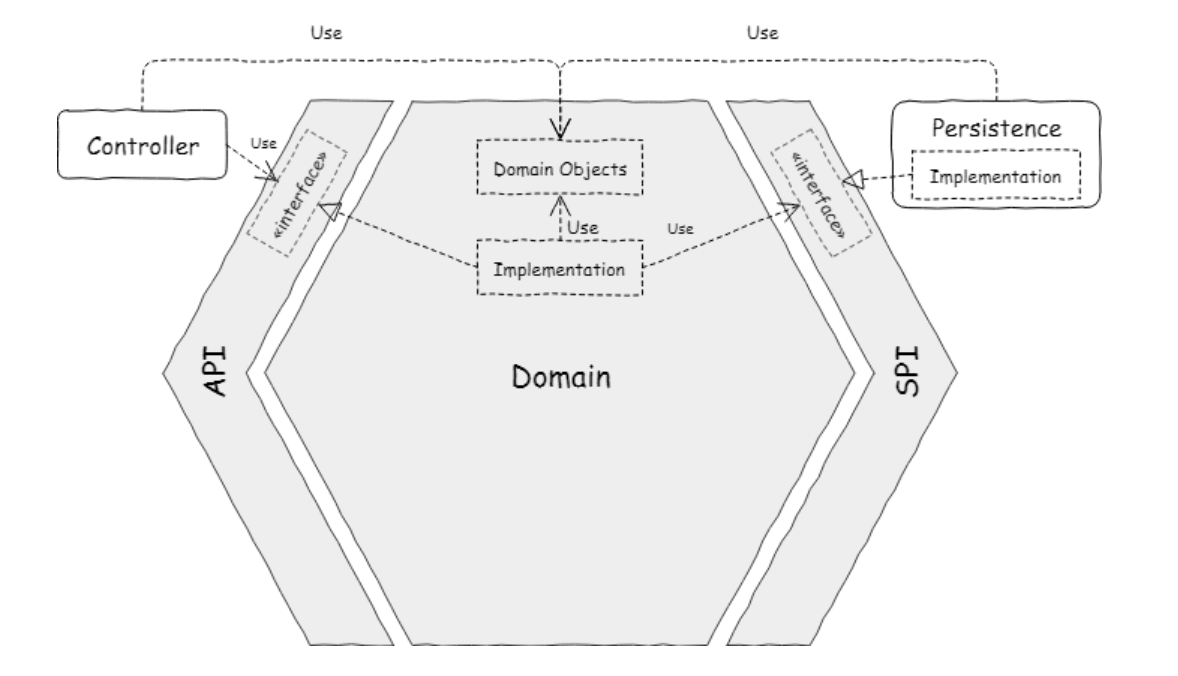
\includegraphics[width=\linewidth]{img/hexagon-dependency.png}
	\caption{Znázornění vzájemných závislostí v hexagonální architektuře (zdroj \cite{beyondxscratch})}
	\label{fig:dependency-hexagon}
\end{figure}
% Vzory typické
% zmínit se o dependency injection pattern - vyžaduje, jelikož se programuje striktně proti interfacům (bergen, campament) + můžu přidat obrázek patternů
Na závěr této sekce je důležité zdůraznit, že přes zmíněné kladné vlastnosti hexagonální architektury existují i záporné. Mezi ně patří především komplexita celého řešení, počet modulů zkrátka roste s počtem portů a adaptérů \cite{hexagonal-this}. Následně můžeme narazit díky komplexitě projektu (závislosti, moduly a podobně) na problémy s výkonem \cite{hexagonal-this} a s komplikovanou správou celého projektu. Jak jsme již zmínili zápory kompenzujeme klady, především dobrou připraveností na změny a testy.

\section{Hexagonální architektura pro náš případ}
V následující sekci shrneme, jak bude v našem případě použita hexagonální architektura. Představíme diagram komponent, doménový model a sekvenční diagramy. Důležité je, že se stále jedná o technologicky nezávislé modely, které popisují obecný návrh systému pro vyhledávání dle kompetencí.\par
\subsection{Komponenty}
Na diagramu komponent, který je součástí přílohy č. \ref{fig:component-model}, vidíme jednotlivé komponenty systému. Závislosti mezi nimi jsou navrženy tak, jak je tomu v hexagonální architektuře.
\subsubsection{Doména}
Jedná se o centrální část systému, která obsahuje doménový model, business logiku aplikace a porty. Na doméně závisí všechny ostatní komponenty aplikace.\par
\paragraph{Doménový model:} Tvoří jádro celého systému, v podstatě se v něm nachází základní entity reálného světa, které jsou v systému namodelovány. Součástí doménového modelu musí být pouze entity, jejich metody a vlastnosti, které nejsou závislé na konkrétním řešení.
Doménový model je součástí přílohy č. \ref{fig:domain-model} a má následující části:
\begin{itemize}
    \item Osoba - entita reprezentující osobu v dané organizaci (v našem případě FEL ČVUT)
    \item Pracoviště - entita reprezentující pracoviště v dané organizaci (v našem případě se jedná o katedry)
    \item Znalost - reprezentuje vazbu mezi osobou a konceptem, přidává jí navíc sílu a poznámku (napříkla jak daná znalost vznikla, resp. odkud jsme jí odvodili)
    \item Koncept - reprezentuje cokoliv, co může být poznáno osobou, jedná se o informace či atomické pojmenované skutečnosti (konkrétní reprezentace je podmíněna konkrétním řešením, domníváme se však, že bez konceptů se v nějaké podobě neobejde žádné řešení); je důležité nezaměňovat tento pojem s ontologickým konceptem, který reprezentuje ontologickou kategorii (viz \ref{ontologies})
    % , v kapitole č. \ref{sec:terms} je tento koncept označen jako \textit{předmět kompetence}
\end{itemize}
V diagramu jsou dále k vidění vazby mezi jednotlivými objekty i s popiskem. 
% Za zmínku stojí hlavně rekurzivní vazba konceptu. Tato vazba nastiňuje existenci sémantické vazby mezi koncepty. Není nutné, aby jí každé řešení muselo mít, v doméně jsme jí však obsáhli - tento druh modelování je v jistém smyslu omezený a není možné vždy striktně oddělit doménu od zbytku systému, který již není tak neměnný. [možná by to chtělo ještě promyslet]
\paragraph{Business logika:}
V této části aplikace jsou typicky k dispozici operace s entitami domény (CRUD) a implementované případy užití (hlavní aplikační logika). Business logika využívá SPI porty a její součástí je implementace API portů.\par
V našem případě se jedná převážně o logiku vyhledávání osob dle kompetencí a operace s tím spojené. V této části se používají SPI adaptéry, které poskytují další služby (například vyhledávání v DB).
\paragraph{Porty a adaptéry:}
Součástí domény jsou API a SPI porty ve formě rozhraní. Dle idey hexagonální architektury je součástí domény zároveň implementace rozhraní API portů.
\subsubsection{API}
V levé části diagramu komponent (\ref{fig:component-model}) je tzv. řídící část hexagonální architektury ve formě API adaptérů. Tyto adaptéry závisí na API portech implementovaných v doméně a volají jejich funkce. V naší aplikaci tyto adaptéry budou představovat typicky REST API případně GraphQL API. Předpokládáme, že tímto způsobem bude aplikace komunikovat s případnými příjemci (v diagramu komponent je takovýto klient také zobrazen). V obrázku lze též vidět, že předpokládáme logické oddělení Knowledge API, umožňující vyhledávání osob a Base API, které umožňuje základní aplikační případy užití (autentizace, případně další týkající se více správy aplikace, než samotného vyhledávání).

\subsubsection{SPI}
Na pravé straně diagramu (\ref{fig:component-model}) je vidět tzv. řízená část hexagonální architektury ve formě SPI adaptérů. Tato část je klíčová z pohledu odolnosti naší architektury vůči změnám použitého řešení. Bez ohledu na to, jaké konkrétní řešení pro vyhledávání dle kompetencí použijeme, domény se to dotkne jen minimálně. Naopak v této části SPI adaptérů, konkrétně u adaptérů zajišťujících samotné vyhledávání, předpokládáme změny. U uživatelských adaptérů (jak jsme je nazvali na obrázku \ref{fig:component-model}), které poskytují spíše aplikační logiku (například přihlašování), opět neočekáváme velké změny, přesto by to bylo možné. V diagramu jsme navrhli několik možných adaptérů, jedná se však pouze o příklady, v konkrétním případě záleží na zvoleném řešení. SPI Adaptéry zajišťují další komunikaci s případnými externími systémy (například databáze, API jiných systémů).\par
% Na diagramu komponent (\ref{fig:component-model}) jsou  na pravé straně zobrazeny databáze (DB), již však není vidět, že tyto databáze nemusí plnit samotná aplikace. U některých řešení se dá předpokládat, že další moduly stávající aplikace, nebo další drobné aplikace případně skripty budou databázi plnit. Plnění databází a celá logika získávání dat pro naše účely je velmi rozsáhlá a komplikovaná, v této práci se jí nezaobíráme. Pochopitelně tato problematika souvisí s transformací dat, kterou jsme zmínili v kapitole č. \ref{chap:processing}.
% [TODO možná moduly lépe namapovat na požadavky z úvodu)]
\subsection{Komunikační sekvence}
Součástí přílohy \ref{appendix:sequence} je diagram sekvencí, na kterém jsme se pokusili demonstrovat, jak bude probíhat komunikace mezi cílovým uživatelem naší aplikace a aplikací samotnou při volání UC1 (\ref{UC1}).
% [odkaz na UC, doplnit asi všude takovéto provázání mezi požadavky, UC apod.]. 
Zároveň je na něm k vidění, jak spolu komunikují jednotlivé komponenty aplikace.\par
Důležité je, že komunikace s aplikací může probíhat synchronně (\ref{fig:sequence-synchronous}) či asynchronně (\ref{fig:sequence-asynchronous}). To jinými slovy znamená, že výsledek hledání může koncový uživatel dostat ihned po dotazu, nebo mu bude navrácen identifikátor hledání a na jeho výsledek se zeptá později. Která varianta bude použita, záleží na zvoleném řešení.\par
% na tom, jak bude zvolené řešení časově náročné. Při delším zpracování není vhodné udržovat mezi oběma stranami synchronní připojení. Existují samozřejmě další faktory, které ovlivňují způsob této komunikace - použití vláken na straně serveru, asynchronní technologie (např. klientský Javascript, který nutně neblokuje webového klienta při další interakci) [TODO: podložit, nebo možná vyhodit, možná tu mluvím o různých věcech]. \par
% Je nezbytné dodat, že diagramy jsou pouze schématické, pro pochopení celého konceptu. Jsou v nich jistě části, které by se dali dotáhnout do větší úrovně detailu, to ale nebylo naším cílem. Naším cílem byla primárně srozumitelnost, jak tomu u diagramů bývá.
% Například SPI adaptérů (na obrázku [odkaz] tzv. adaptéry konkrétního řešení) může být několik a domény s každým z nich může komunikovat zvlášť. Ve většině případů lze vždy ještě nalézt výjimečné stavy (neúspěch při připojení do databáze apod.), které v diagramu pro zvýšení přehlednosti nejsou zohledněné. V neposlední řadě není zmíněno, že při asynchronním zpracování se uživatel může API zeptat na výsledek dříve než jej bude mít k dispozici. V takovém případě API vrátí zvoleným způsobem zprávu "vyhledávání stále probíhá".
\section{Shrnutí}
V této sekci jsme se zabývali návrhem systému pro vyhledávání osob dle jejich kompetencí. Začali jsme od cílů, požadavků a případů užití a pokračovali jsme až k detailnímu popisu zvolené architektury. V následující sekci na náš návrh navážeme popisem implementace prototypu.







% [diagram nasazení - technologicky nezávislý - nejspíš ne]

% - zamyslet se nad platnými pravidly, případně praktikovat reasoning
% - Vytvořit testovací data
% - Vložit do graphDB




% i.	Architektura aplikace – požadavek na modularitu a obecnost (nejdříve obecně, bez technologií
% \section{Hexagonální architektura - Porty a adaptéry}
% Architektura (udělat diagram komponent pro mé konkrétní použití)
% - Hexagonal (Port and Adapter)
% https://github.com/gshaw-pivotal/spring-hexagonal-example
% https://blog.octo.com/en/hexagonal-architecture-three-principles-and-an-implementation-example/
% - vložit obrázek z citovaného zdroje